\section{Конструкторский раздел}
%В этом разделе будет приведено проектирование базы данных и проектирование приложения.
%Также будет спроектирован триггер, осуществляющие автоматически пересчитывать рейтинга турнира при добавлении новых оценок.
\subsection{Критерия для распределения поездов}
Все поезда должны соответствовать следующим критериям:
\begin{itemize}
	\item на одной пути интервал между двумя поездами --- 10 минут;
	\item если все нет свободных платформ, поезд задерживается.
\end{itemize}
\subsection{Разработка алгоритма}

На рисунке \ref{img:schedule} приведена схема алгоритма распределения поездов, сделанная студентом Фам Минь Хиеу.

\begin{figure}[h]
	\centering
	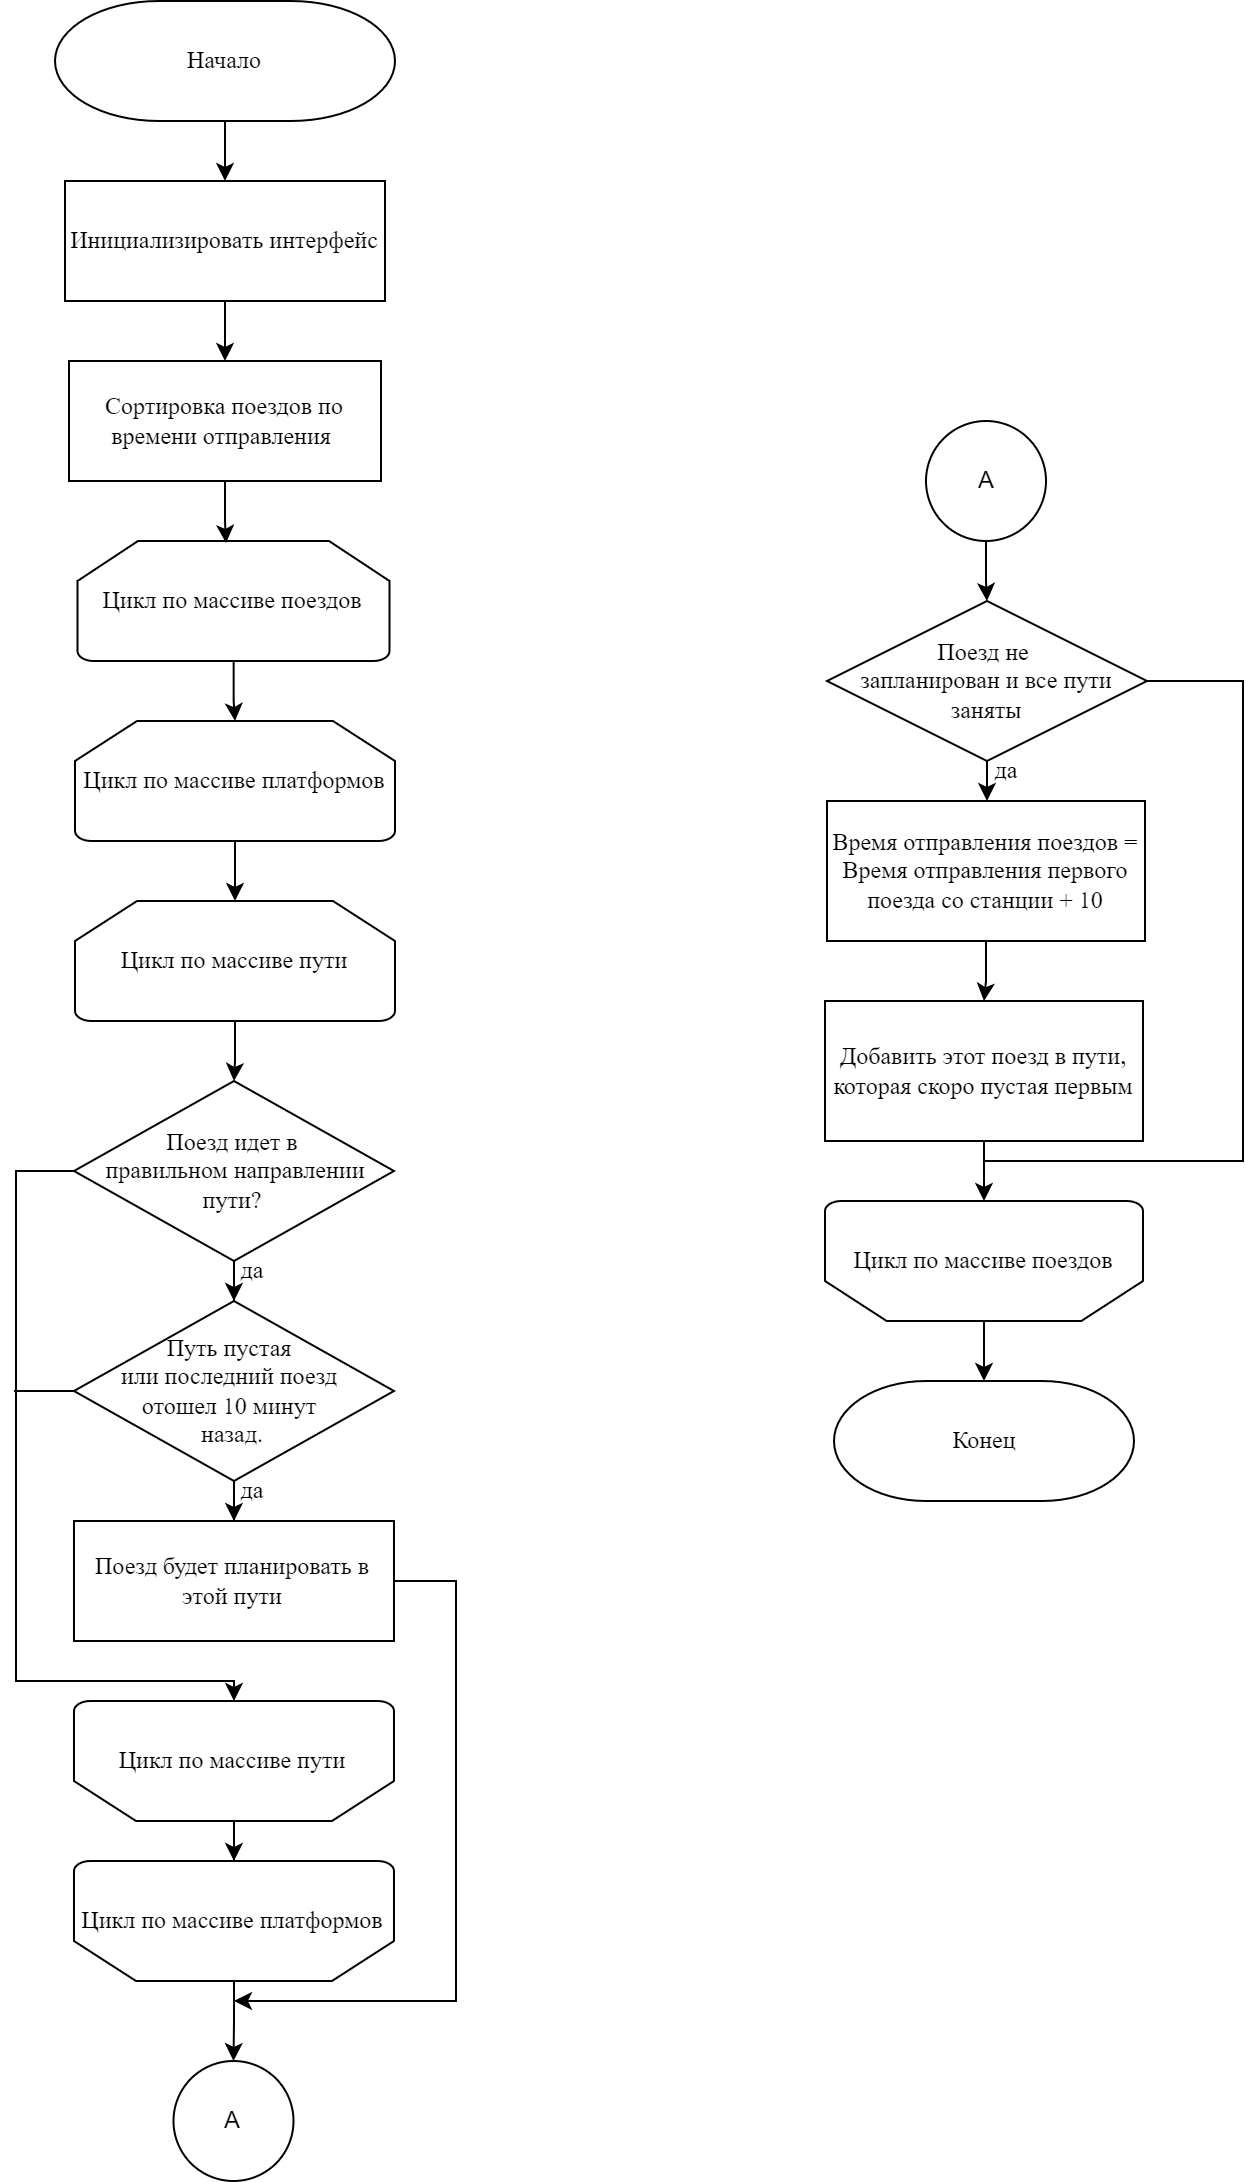
\includegraphics[height=0.7\textheight]{img/schedule.png}
	\caption{Алгоритм распределения поездов}
	\label{img:schedule}
\end{figure}